\section{API Endpoint Specification}
\label{appendix:api-endpoints}

This appendix provides the technical specification for the API. It includes a visual overview of all available endpoints and detailed examples of the contracts for key operations.

\subsection{API Endpoints Overview}

The following Figure \ref{fig:api-endpoints-overview-appendix}, generated by the Swagger UI tool, provides a complete list of all endpoints supported by the backend API. 

\begin{figure}[H]
    \centering
    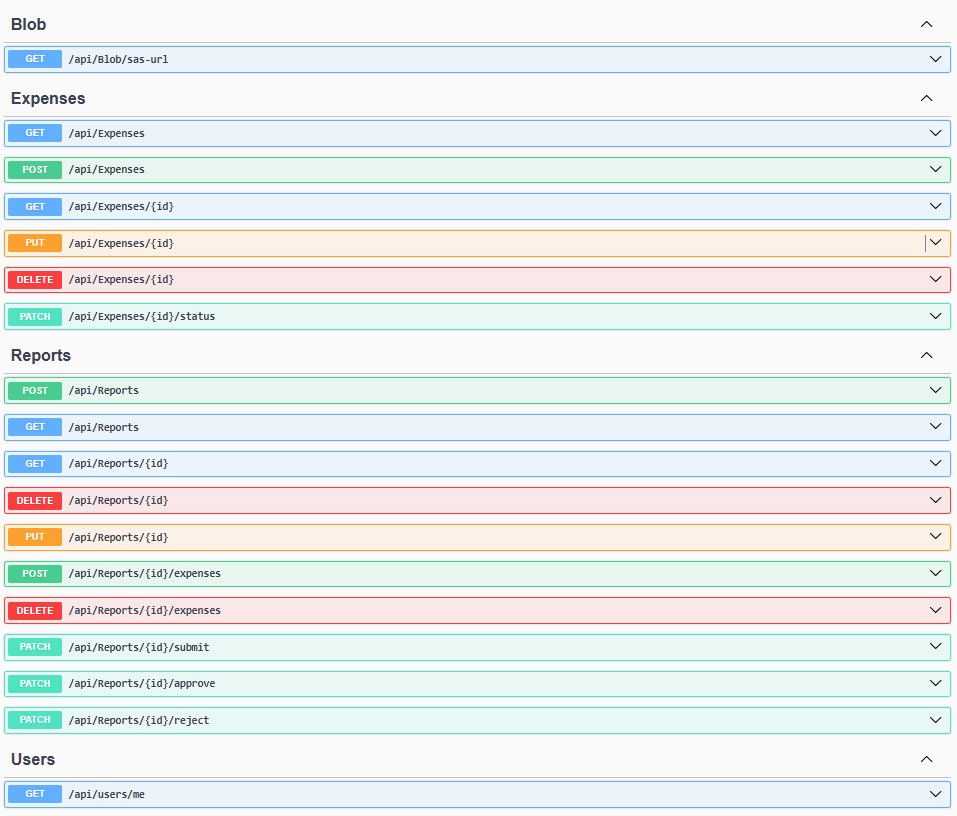
\includegraphics[width=\textwidth]{Images/swagger/APIendpoints1.png}
    \caption[Complete endpoints  list generated by Swagger UI]
    {Complete endpoints  list generated by Swagger UI. [Own creation]}
    \label{fig:api-endpoints-overview-appendix}
\end{figure}


\subsection{Detailed Endpoint Examples}

To illustrate the structure of the API contracts, this section provides the full specification for two critical endpoints.

\subsubsection{Upload a New Expense}

This endpoint is used to upload a new expense receipt and create the initial record in the system. It is the entry point for the asynchronous AI processing flow. Figure \ref{fig:upload-expense-input-appendix} shows the request body specification, while Figure \ref{fig:upload-expense-response-appendix} depicts the response schemas for this concrete endpoint.

\begin{figure}[H]
    \centering
    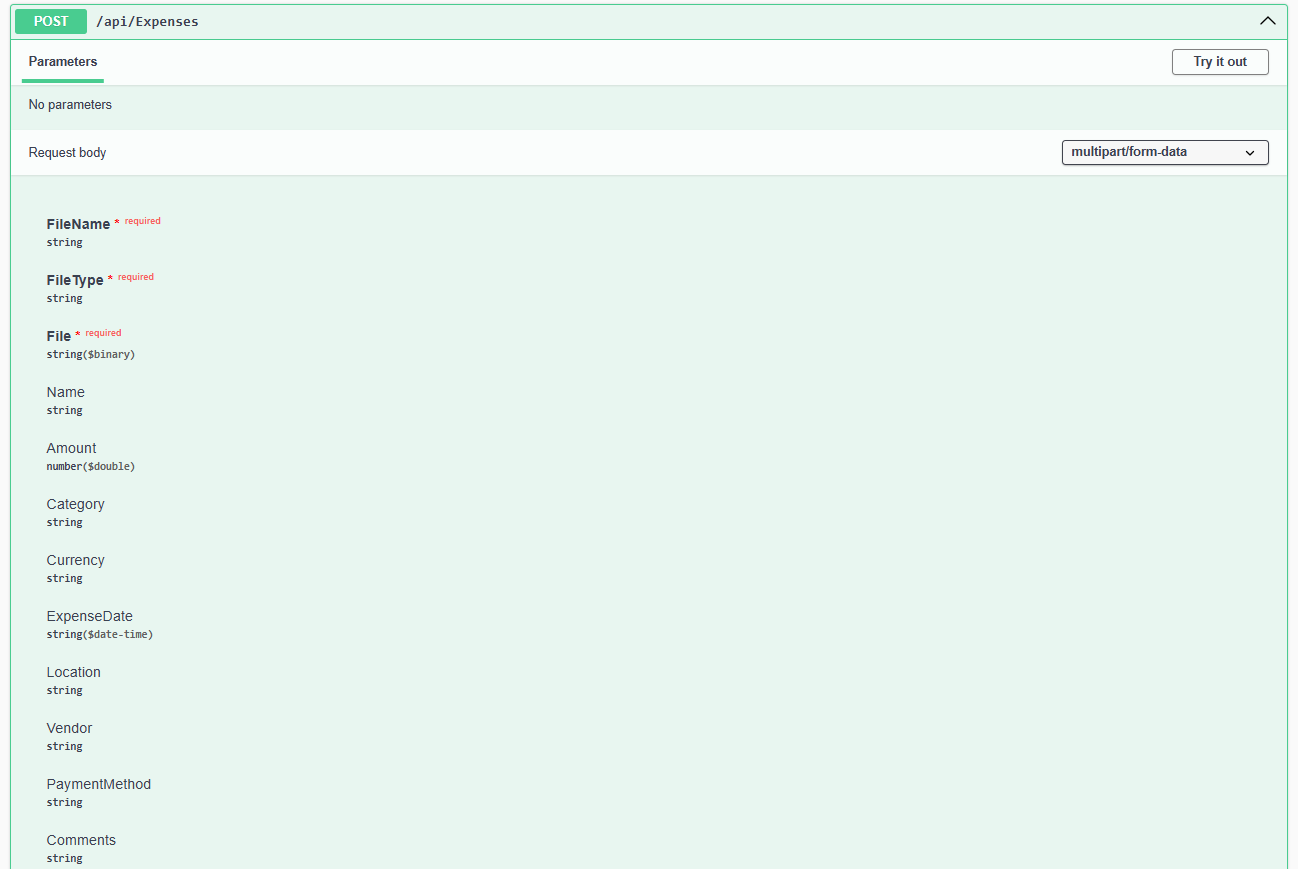
\includegraphics[width=\textwidth]{Images/swagger/upload_expense_input.png}
    \caption[Request body specification for the Upload Expense endpoint]
    {Request body specification for the Upload Expense endpoint. [Own creation]}
    \label{fig:upload-expense-input-appendix}
\end{figure}


\begin{figure}[H]
    \centering
    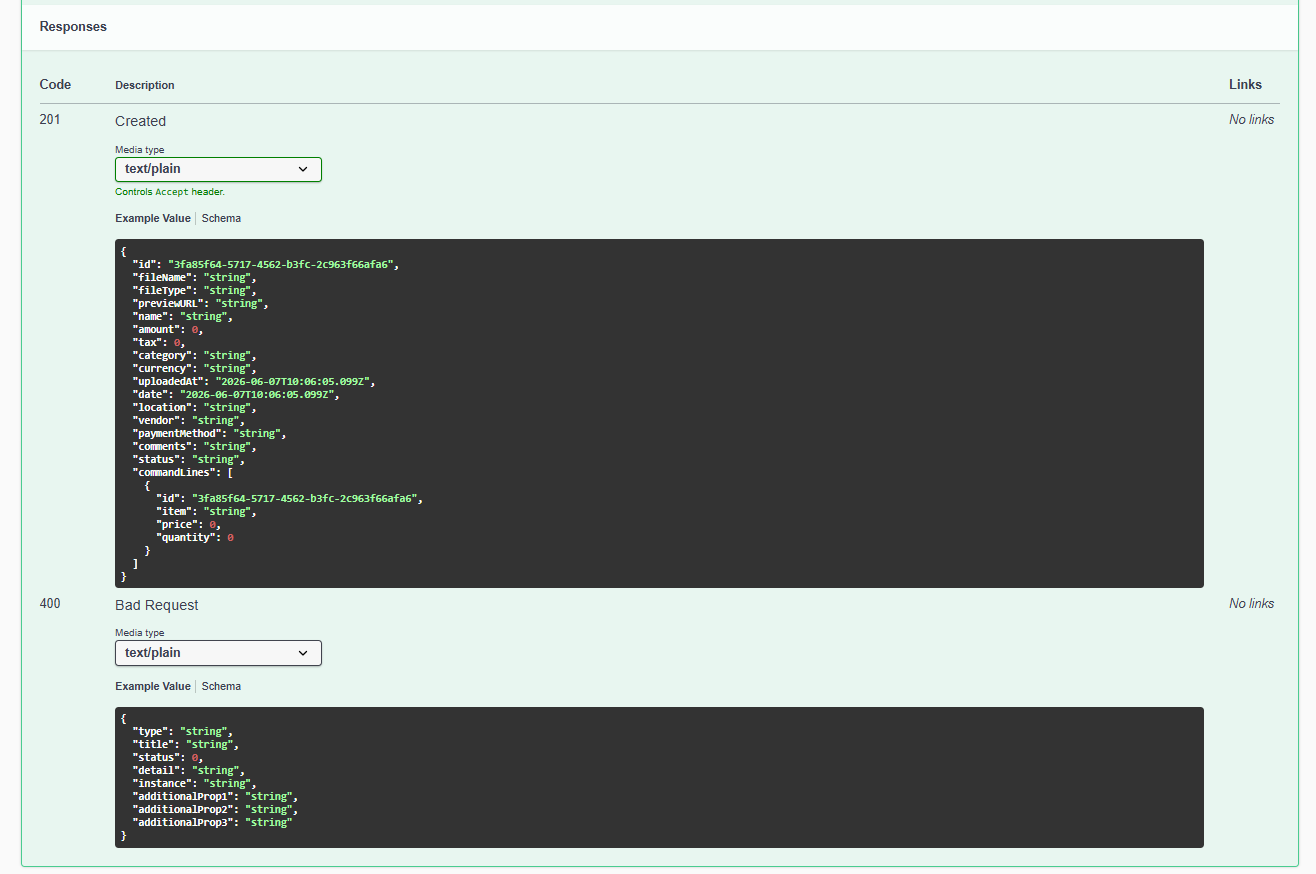
\includegraphics[width=\textwidth]{Images/swagger/upload_expense_response.png}
    \caption[Response schemas for the Upload Expense endpoint]
    {Response schemas for the Upload Expense endpoint. [Own creation]}
    \label{fig:upload-expense-response-appendix}
\end{figure}


\subsubsection{Approve a Report}

This endpoint manages a key business workflow, allowing a user with administrative privileges to approve a submitted expense report. Both request body and response specifications are depicted in Figure \ref{fig:approve-report-input-appendix}.

\begin{figure}[H]
    \centering
    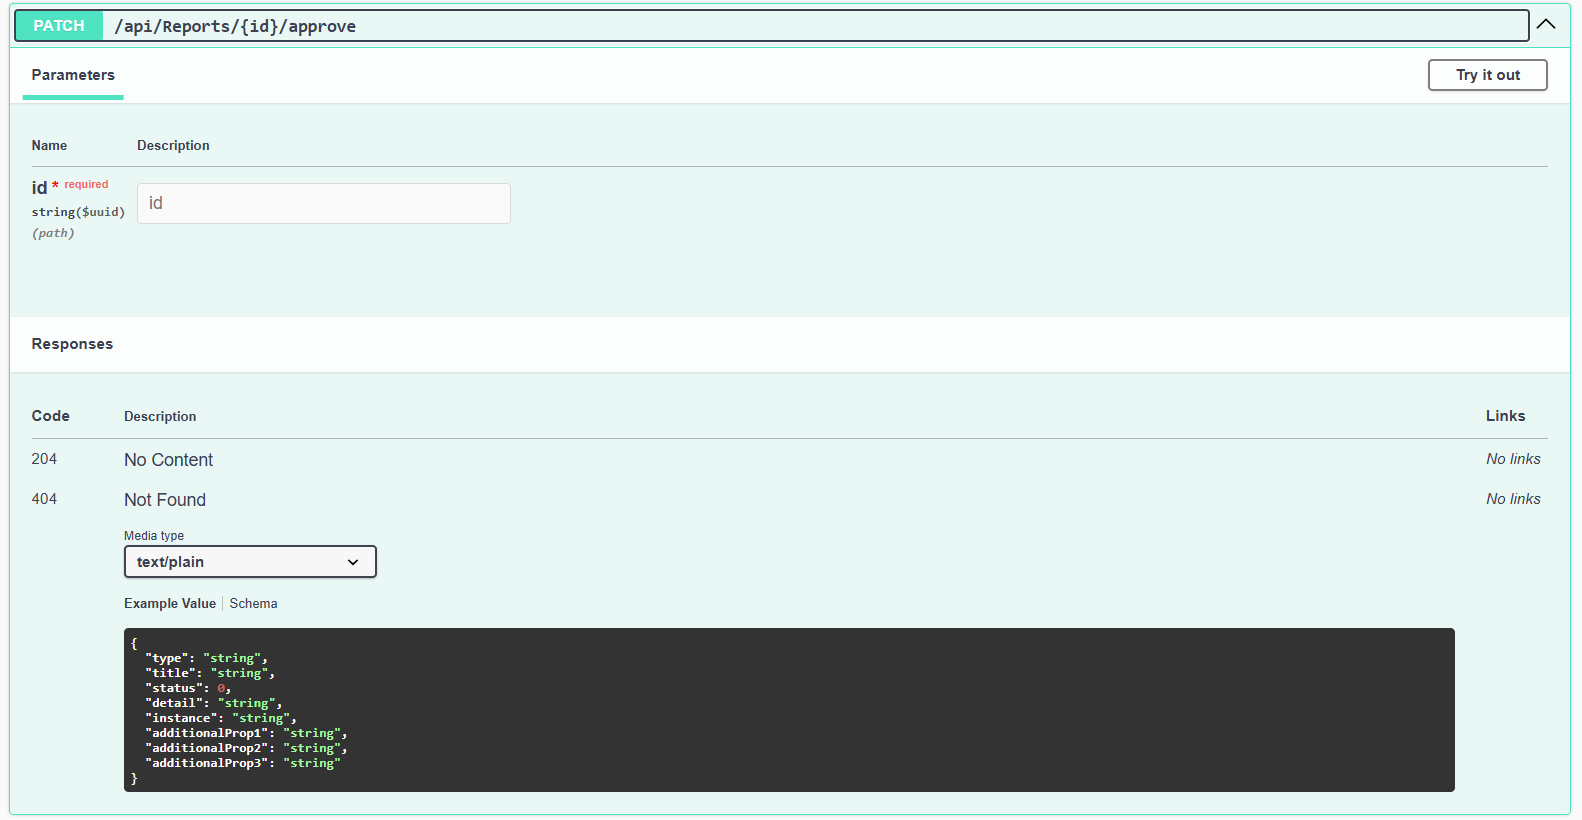
\includegraphics[width=\textwidth]{Images/swagger/ApproveReportEspecification.png}
    \caption[Complete specification for the Approve Report endpoint]
    {Complete specification for the Approve Report endpoint. [Own creation]}
    \label{fig:approve-report-input-appendix}
\end{figure}
